% Latex template: https://github.com/mqTeXUsers/Macquarie-University-Beamer-Theme

% Slide Masters:

% Title
% Text
% 2 column
% Full-image
% Bibliography
% Closing
 
\documentclass[aspectratio=169, 11pt]{beamer} % Aspect ratio
% https://tex.stackexchange.com/a/14339/5483 
% Possible values: 1610, 169, 149, 54, 43 and 32.
% 169 = 16:9

\PassOptionsToPackage{table}{xcolor}    %https://tex.stackexchange.com/a/5365/5483

\usetheme{macquarie}
\usepackage{multicol} % https://tex.stackexchange.com/a/396018/5483
\usepackage{xurl}
\usepackage[british]{babel}       % Set language
% \usepackage[utf8x]{inputenc}      % Set encoding
\usepackage{colortbl}
\mode<presentation>           % Set options
{
  \usetheme{default}          % Set theme
  \usecolortheme{default}         % Set colors
  \usefonttheme{default}          % Set font theme
  \setbeamertemplate{caption}[numbered] % Set caption to be numbered
}

% Uncomment this to have the outline at the beginning of each section highlighted.
%\AtBeginSection[]
%{
%  \begin{frame}{Outline}
%    \tableofcontents[currentsection]
%  \end{frame}
%}

\usepackage{graphicx}         % For including figures
\usepackage{booktabs}         % For table rules
\usepackage{hyperref}         % For cross-referencing


\usepackage{enumitem} % https://tex.stackexchange.com/a/2292/5483

%https://tex.stackexchange.com/a/371844/5483
\setbeamerfont{bibliography entry author}{size=\tiny}
\setbeamerfont{bibliography entry title}{size=\tiny}
\setbeamerfont{bibliography entry location}{size=\tiny}
\setbeamerfont{bibliography entry note}{size=\tiny}
\setbeamerfont{bibliography item}{size=\tiny}

%https://tex.stackexchange.com/q/333587/5483
%TODO SHAWN REPLACE OSF URL
%\setbeamertemplate{footline}{\strut~\texttt{https://github.com/MQ-FOAR705/MQ-FOAR705-Week1}\hfill\insertframenumber~/~\inserttotalframenumber\strut~~~}

\title{FOAR705 Learning Journals and Week 2 Slides} % Presentation title
\author{Brian Ballsun-Stanton | Shawn A Ross | Kathryn Elliot}               % Presentation author
\institute{Faculty of Arts}         % Author affiliation
\date{Friday 09 August 2019}                 % Today's date  
\begin{document}

% Title page
% This page includes the informations defined earlier including title, author/s, affiliation/s and the date
% \begin{frame}[noframenumbering]

\maketitle

  
% \end{frame}


\section{Intentions of the Learning Journal}

\begin{frame}{Learning Journals}
\begin{itemize}[label=\textbullet]
    \item To serve as a Labroatory Notebook -- a record of:
    \begin{itemize}
        \item Thoughts
        \item Intentions
        \item Results
    \end{itemize}
    \item Mechanism for showing your work
    \item Reminders of common mistakes and solutions
    \item Demonstration of growth over time
\end{itemize}    
\end{frame}

\begin{frame}{Grading Rubric}
\begin{itemize}[label=\textbullet]
    \item Exercise Documentation (70\letterpercent{})
    \item Committing your work (10\letterpercent{})
    \item Error Reflection and Solution (20\letterpercent{})
\end{itemize}    
\end{frame}


% Outline
% This page includes the outline (Table of content) of the presentation. All sections and subsections will appear in the outline by default.
% \begin{frame}{The context of Research Data Management}
%   \tableofcontents
% \end{frame}

% % The following is the most frequently used slide types in beamer
% % The slide structure is as follows:
% %
% %\begin{frame}{<slide-title>}
% % <content>
% %\end{frame}

% \section{Code of Conduct}

% \begin{frame}{Unit Code of Conduct}
% This class is using a great deal of material from The Carpentries. All interactions related to this class, inside and outside, abide by The Carpentries Code of Conduct.

% Report code of conduct violations to Shawn, Brian, or eresearch@mq.edu.au.

% \url{https://docs.carpentries.org/topic_folders/policies/code-of-conduct.html}

% In summary, we want to emphasise:

% \begin{itemize}[label=\textbullet]
%     \item Use welcoming and inclusive language
%     \item Be respectful of different viewpoints and experiences
%     \item Gracefully accept constructive criticism
%     \item Focus on what is best for the community
%     \item Show courtesy and respect towards other community members
% \end{itemize}

% \end{frame}

% \section{Expectations}

% \begin{frame}{Is the content 'too hard'?}
%  `I still have my concerns about how over-technical this course is given it is now meant to be taken by students from across the entire Faculty from diverse backgrounds and with diverse interests...I suspect will cause students anxiety and maybe lead to drop out.'
%     \begin{itemize}[label=\textbullet]
%         \item Before we start, what was your reaction to reading the Unit description?
%         \item Do you agree with the quote above?
%     \end{itemize}
% \end{frame}

% \begin{frame}{Expectations and workload}
%   You are undertaking an Masters of Research at a top one-percent university (QS ranking 125 in Arts and Humanities, 202 in Social Sciences). Expectations and workload higher than what you are accustomed to.
%     \begin{itemize}[label=\textbullet]
%         \item Expect a workload of six hours per week outside of class to earn a DN or HD.
%         \item Avoid missing classes. If you do, expect to spend four hours to catch up.
%         \item If you want to continue to a PhD you need to maintain a DN or HD average.
%         \item Both of us have taught overseas and are engaged with international trends in research technology. This unit has been calibrated to the international environment.
%         \item Considering the academic job market, competition is fierce.
%         \item Most of you will not get academic jobs, so transferable skills are crucial.
%         \item It is our job to prepare you for this environment, and yours to make yourself competitive.
%     \end{itemize}
% \end{frame}

% \begin{frame}{Assessment}

% \begin{itemize}[label=\textbullet]
%     \item Proof of Concept
%     \item Original Software Publication
%     \item Lightning talk
%     \item Learning journal
% \end{itemize}

% \end{frame}

% \section{Don't panic!}

% \begin{frame}{Data Carpentry: a proven approach}
%     `Building communities teaching universal data literacy'
       
%     `Data Carpentry trains researchers in the core data skills for efficient, shareable, and reproducible research practices. We run accessible, inclusive training workshops; teach openly available, high-quality, domain-tailored lessons; and foster an active, inclusive, diverse instructor community that promotes and models reproducible research as a community norm.' \cite{Teal2016-gy}

%     `Since 1998, Software Carpentry has been teaching researchers the computing skills they need to get more done in less time and with less pain. Our volunteer instructors have run hundreds of events for more than 34,000 researchers since 2012.' \cite{Duckles2018-fu}
% \end{frame}

% \begin{frame}{Data Carpentry: widely used worldwide in HASS}
%     Carpentries training is used all over the world to teach digital literacy and computational thinking to Humanities and Social Sciences students and researchers.
%     \begin{itemize}[label=\textbullet]
%         \item Digital Humanities at Oxford Summer School
%         \item CODATA-RDA School of Research Data Science
%         \item Australian Research Data Cloud training
%         \item THATCamps (e.g., at Sydney ResBaz 2019)
%     \end{itemize}
% \end{frame}

% \begin{frame}{Data Carpentry: used at Macquarie}
%   Other MRes students at this university have successfully undergone DC training:
%     \begin{itemize}[label=\textbullet]
%         \item BIOL703 Research Skills for Biology
%         \item No excess attrition, high student satisfaction, good feedback
%         \item Nominated for a Vice-Chancellor's Learning and Teaching award
%         \item Is the background or needs of Arts students that different from ecology, biology, environmental sciences, and related fields?
%     \end{itemize}
% \end{frame}

% \begin{frame}{Previous HASS MRes students have thrived}
%   \url{https://www.youtube.com/watch?v=r9jpe9_2z3c}
% \end{frame}

% \section{What, and why?}

% \begin{frame}{Digital literacy: creators, not consumers}
%     \begin{figure}[H]
%         \centering
%         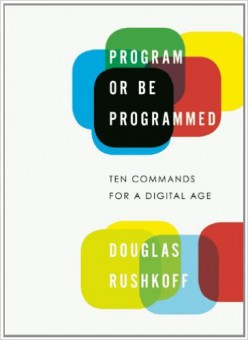
\includegraphics[height=.6\textheight]{figures/2011-ProgOrBeProgged-248x340.jpg}
%         \caption{Program or be Programmed, Douglas Rushkoff}
%         \label{fig:programmed}
%     \end{figure}
  
%   See also: \url{https://impossiblehq.com/an-unexpected-ass-kicking/}
% %insert 'Program or be programmed' book cover image, and link to 'An unexpected ass kicking' %https://rushkoff.com/books/program-or-be-programmed/
% %https://impossiblehq.com/an-unexpected-ass-kicking/

% \end{frame}

% \begin{frame}{Computational thinking: what can you do with a computer?}
% \begin{figure}[H]
%         \centering
%         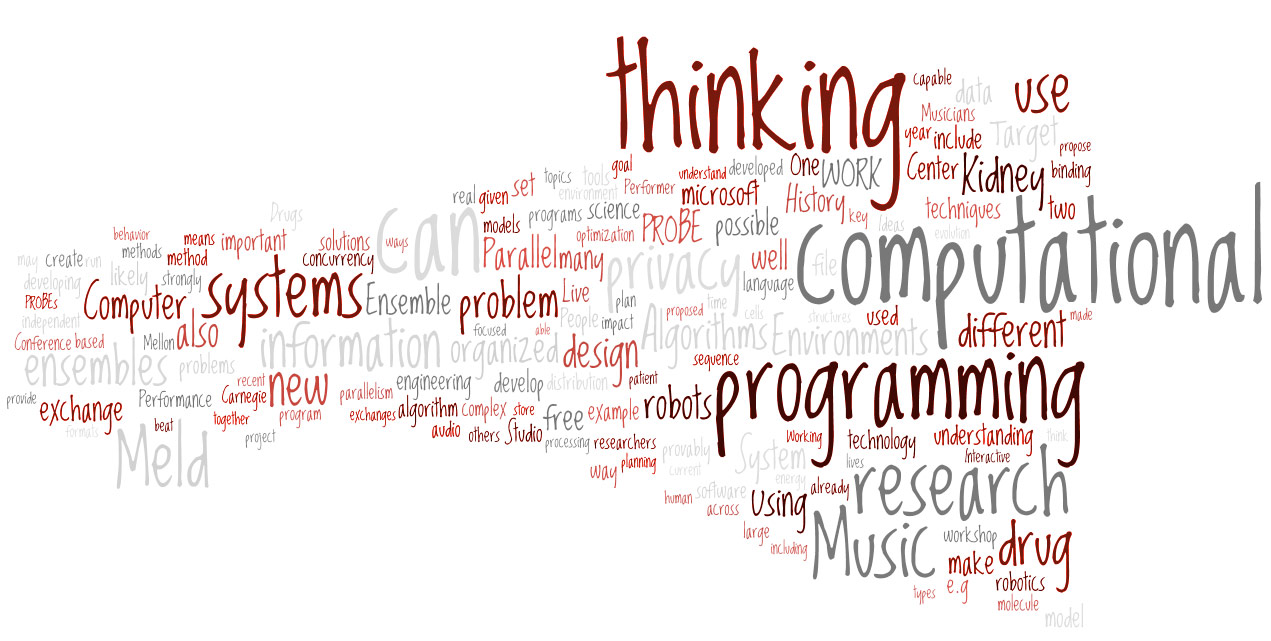
\includegraphics[height=.6\textheight]{figures/ctc-w2b.jpg}
%         \caption{'To flourish in today's world, computational thinking has to be a fundamental part of the way people think and understand the world.' \cite{Center_for_Computational_Thinking2012-tt}}
%         \label{fig:ctc}
%     \end{figure}
% %insert https://www.cs.cmu.edu/~CompThink/images/ctc-w2b.jpg
% %caption: 'To flourish in today's world, computational thinking has to be a fundamental part of the way people think and understand the world.' https://www.cs.cmu.edu/~CompThink/

% \end{frame}

% \begin{frame}{Tools and approaches}
% Only within these frameworks can you use available tools and approaches - but we will introduce you to a range of them, customised to the disciplinary mix in the class.
%     \begin{itemize}[label=\textbullet]
%         \item Research design and project management
%         \item Data management planning
%         \item Data capture
%         \item Data analysis and collaboration
%         \item Data archiving and dissemination
%     \end{itemize}

% \end{frame}


% \section{Tools and Communication}
% \begin{frame}{Discussion on which tools we will use as a class}

% \begin{itemize}[label=\textbullet]
%     \item Chat/coordination/project management software
%     \item Typesetting software
%     \item Version control online repository
%     \item File sharing mechanisms
%     \item Backup mechanisms
% \end{itemize}

% \end{frame}

% \begin{frame}{Coordination outside of class}

% \begin{itemize}[label=\textbullet]
%     \item Hacky-hour/study groups: \url{https://science.mozilla.org/programs/studygroups}
%     \item Consultation Hours: Friday 12:45-1:45pm (AHH Level 2 lobby) and 4:15-5:15pm, campus hub (before and after seminar)
%     \item \url{https://twitter.com/Rusers_MQ}
% \end{itemize}

% \end{frame}

% \section{Moving on to Data Carpentry}


% \begin{frame}{Pre-Carpentry survey}

% At the start and end of every carpentries workshop, we poll participants.

% \url{https://bit.ly/FOAR705-pre}

% \begin{figure}[H]
%         \centering
%         
\includegraphics[height=.6\textheight]{figures/qr.jpeg}
%         \caption{\url{https://mqedu.qualtrics.com/jfe/form/SV_5v6iQJSBZDNhq4d?workshop=FOAR705-2019}}
%         \label{fig:foarqr}
%     \end{figure}
    
% \end{frame}

% \begin{frame}{Sticky notes}

% We use sticky notes during our workshops (and thus during our classes) to indicate progress or needs for assistance. 

% We also use them as minute cards for feedback and the end of each session. 

% \end{frame}
% \begin{frame}{Starting the workshop}
%     \begin{itemize}
%         \item \url{https://datacarpentry.org/socialsci-workshop/}
%         \item \url{https://datacarpentry.org/spreadsheets-socialsci/setup.html}
%         \item \url{https://datacarpentry.org/openrefine-socialsci/setup.html}
%         \item \url{https://datacarpentry.org/r-socialsci/setup.html}
%     \end{itemize}
% \end{frame}


% % \bibliographystyle{apalike}

% % Adding the option 'allowframebreaks' allows the contents of the slide to be expanded in more than one slide.
% % The "1" comes from the outer theme"


% \section{Minute cards!}
% \begin{frame}{Feedback time}

% On your green sticky, write one thing we did well today.

% On your red sticky, write one thing we could improve upon for next time. Be specific. 

% \end{frame}

% \section{References}

% \begin{multicols}{2}[]
% \bibliography{references}
% \bibliographystyle{apalike}
% \end{multicols}


% \begin{frame}[allowframebreaks]{References}
  
%   \bibliography{references}
%   \bibliographystyle{apalike}
% \end{frame}


\begin{frame}{Thank you!}

% This presentation is available at:
% \texttt{https://osf.io/...}

Source code for this presentation is available at: \url{https://github.com/MQ-FOAR705/MQ-FOAR705-Week2}

This work is licensed under a Creative Commons Attribution 4.0 International License.

\end{frame}



\end{document}